% Options for packages loaded elsewhere
\PassOptionsToPackage{unicode}{hyperref}
\PassOptionsToPackage{hyphens}{url}
%
\documentclass[
  11pt,
  ignorenonframetext,
]{beamer}
\usepackage{pgfpages}
\setbeamertemplate{caption}[numbered]
\setbeamertemplate{caption label separator}{: }
\setbeamercolor{caption name}{fg=normal text.fg}
\beamertemplatenavigationsymbolsempty
% Prevent slide breaks in the middle of a paragraph
\widowpenalties 1 10000
\raggedbottom
\setbeamertemplate{part page}{
  \centering
  \begin{beamercolorbox}[sep=16pt,center]{part title}
    \usebeamerfont{part title}\insertpart\par
  \end{beamercolorbox}
}
\setbeamertemplate{section page}{
  \centering
  \begin{beamercolorbox}[sep=12pt,center]{part title}
    \usebeamerfont{section title}\insertsection\par
  \end{beamercolorbox}
}
\setbeamertemplate{subsection page}{
  \centering
  \begin{beamercolorbox}[sep=8pt,center]{part title}
    \usebeamerfont{subsection title}\insertsubsection\par
  \end{beamercolorbox}
}
\AtBeginPart{
  \frame{\partpage}
}
\AtBeginSection{
  \ifbibliography
  \else
    \frame{\sectionpage}
  \fi
}
\AtBeginSubsection{
  \frame{\subsectionpage}
}
\usepackage{amsmath,amssymb}
\usepackage{lmodern}
\usepackage{iftex}
\ifPDFTeX
  \usepackage[T1]{fontenc}
  \usepackage[utf8]{inputenc}
  \usepackage{textcomp} % provide euro and other symbols
\else % if luatex or xetex
  \usepackage{unicode-math}
  \defaultfontfeatures{Scale=MatchLowercase}
  \defaultfontfeatures[\rmfamily]{Ligatures=TeX,Scale=1}
\fi
\usetheme[]{metropolis}
% Use upquote if available, for straight quotes in verbatim environments
\IfFileExists{upquote.sty}{\usepackage{upquote}}{}
\IfFileExists{microtype.sty}{% use microtype if available
  \usepackage[]{microtype}
  \UseMicrotypeSet[protrusion]{basicmath} % disable protrusion for tt fonts
}{}
\makeatletter
\@ifundefined{KOMAClassName}{% if non-KOMA class
  \IfFileExists{parskip.sty}{%
    \usepackage{parskip}
  }{% else
    \setlength{\parindent}{0pt}
    \setlength{\parskip}{6pt plus 2pt minus 1pt}}
}{% if KOMA class
  \KOMAoptions{parskip=half}}
\makeatother
\usepackage{xcolor}
\newif\ifbibliography
\usepackage{color}
\usepackage{fancyvrb}
\newcommand{\VerbBar}{|}
\newcommand{\VERB}{\Verb[commandchars=\\\{\}]}
\DefineVerbatimEnvironment{Highlighting}{Verbatim}{commandchars=\\\{\}}
% Add ',fontsize=\small' for more characters per line
\newenvironment{Shaded}{}{}
\newcommand{\AlertTok}[1]{\textcolor[rgb]{1.00,0.00,0.00}{\textbf{#1}}}
\newcommand{\AnnotationTok}[1]{\textcolor[rgb]{0.38,0.63,0.69}{\textbf{\textit{#1}}}}
\newcommand{\AttributeTok}[1]{\textcolor[rgb]{0.49,0.56,0.16}{#1}}
\newcommand{\BaseNTok}[1]{\textcolor[rgb]{0.25,0.63,0.44}{#1}}
\newcommand{\BuiltInTok}[1]{#1}
\newcommand{\CharTok}[1]{\textcolor[rgb]{0.25,0.44,0.63}{#1}}
\newcommand{\CommentTok}[1]{\textcolor[rgb]{0.38,0.63,0.69}{\textit{#1}}}
\newcommand{\CommentVarTok}[1]{\textcolor[rgb]{0.38,0.63,0.69}{\textbf{\textit{#1}}}}
\newcommand{\ConstantTok}[1]{\textcolor[rgb]{0.53,0.00,0.00}{#1}}
\newcommand{\ControlFlowTok}[1]{\textcolor[rgb]{0.00,0.44,0.13}{\textbf{#1}}}
\newcommand{\DataTypeTok}[1]{\textcolor[rgb]{0.56,0.13,0.00}{#1}}
\newcommand{\DecValTok}[1]{\textcolor[rgb]{0.25,0.63,0.44}{#1}}
\newcommand{\DocumentationTok}[1]{\textcolor[rgb]{0.73,0.13,0.13}{\textit{#1}}}
\newcommand{\ErrorTok}[1]{\textcolor[rgb]{1.00,0.00,0.00}{\textbf{#1}}}
\newcommand{\ExtensionTok}[1]{#1}
\newcommand{\FloatTok}[1]{\textcolor[rgb]{0.25,0.63,0.44}{#1}}
\newcommand{\FunctionTok}[1]{\textcolor[rgb]{0.02,0.16,0.49}{#1}}
\newcommand{\ImportTok}[1]{#1}
\newcommand{\InformationTok}[1]{\textcolor[rgb]{0.38,0.63,0.69}{\textbf{\textit{#1}}}}
\newcommand{\KeywordTok}[1]{\textcolor[rgb]{0.00,0.44,0.13}{\textbf{#1}}}
\newcommand{\NormalTok}[1]{#1}
\newcommand{\OperatorTok}[1]{\textcolor[rgb]{0.40,0.40,0.40}{#1}}
\newcommand{\OtherTok}[1]{\textcolor[rgb]{0.00,0.44,0.13}{#1}}
\newcommand{\PreprocessorTok}[1]{\textcolor[rgb]{0.74,0.48,0.00}{#1}}
\newcommand{\RegionMarkerTok}[1]{#1}
\newcommand{\SpecialCharTok}[1]{\textcolor[rgb]{0.25,0.44,0.63}{#1}}
\newcommand{\SpecialStringTok}[1]{\textcolor[rgb]{0.73,0.40,0.53}{#1}}
\newcommand{\StringTok}[1]{\textcolor[rgb]{0.25,0.44,0.63}{#1}}
\newcommand{\VariableTok}[1]{\textcolor[rgb]{0.10,0.09,0.49}{#1}}
\newcommand{\VerbatimStringTok}[1]{\textcolor[rgb]{0.25,0.44,0.63}{#1}}
\newcommand{\WarningTok}[1]{\textcolor[rgb]{0.38,0.63,0.69}{\textbf{\textit{#1}}}}
\usepackage{graphicx}
\makeatletter
\def\maxwidth{\ifdim\Gin@nat@width>\linewidth\linewidth\else\Gin@nat@width\fi}
\def\maxheight{\ifdim\Gin@nat@height>\textheight\textheight\else\Gin@nat@height\fi}
\makeatother
% Scale images if necessary, so that they will not overflow the page
% margins by default, and it is still possible to overwrite the defaults
% using explicit options in \includegraphics[width, height, ...]{}
\setkeys{Gin}{width=\maxwidth,height=\maxheight,keepaspectratio}
% Set default figure placement to htbp
\makeatletter
\def\fps@figure{htbp}
\makeatother
\setlength{\emergencystretch}{3em} % prevent overfull lines
\providecommand{\tightlist}{%
  \setlength{\itemsep}{0pt}\setlength{\parskip}{0pt}}
\setcounter{secnumdepth}{-\maxdimen} % remove section numbering
\ifLuaTeX
  \usepackage{selnolig}  % disable illegal ligatures
\fi
\IfFileExists{bookmark.sty}{\usepackage{bookmark}}{\usepackage{hyperref}}
\IfFileExists{xurl.sty}{\usepackage{xurl}}{} % add URL line breaks if available
\urlstyle{same} % disable monospaced font for URLs
\hypersetup{
  pdftitle={Pruebas de hipótesis},
  pdfauthor={Gerardo Martín},
  hidelinks,
  pdfcreator={LaTeX via pandoc}}

\title{Pruebas de hipótesis}
\author{Gerardo Martín}
\date{2022-06-29}

\begin{document}
\frame{\titlepage}

\hypertarget{recordatorio}{%
\section{Recordatorio}\label{recordatorio}}

\begin{frame}{¿Qué es una hipótesis?}
\protect\hypertarget{quuxe9-es-una-hipuxf3tesis}{}
\begin{itemize}
\item
  Aseveración que deber ser demostrada
\item
  Hay diferentes tipos de hipótesis, las del área de estudio y las
  estadísticas
\item
  Las estadísticas están relacionadas con algún experimento diseñado
  para demostrar el fenómeno de interés
\end{itemize}
\end{frame}

\begin{frame}{Ejemplo}
\protect\hypertarget{ejemplo}{}
\begin{itemize}
\tightlist
\item
  Hipótesis biológica
\end{itemize}

``Los sapos \emph{Rhinella marina} se benefician de los cuerpos de agua
temporales''

\begin{itemize}
\tightlist
\item
  Estudio diseñado para probar hipótesis biológica:
\end{itemize}

``Se identifican cuerpos de agua permanentes y temporales para ser
vigilados durante temporada de secas y lluvias para contar el número de
renacuajos de \emph{Rhinella marina}''

\begin{itemize}
\tightlist
\item
  Hipótesis estadística:
\end{itemize}

``El número promedio de renacuajos por cuerpo de agua será mayor en
época de lluvias''
\end{frame}

\begin{frame}{Ejemplo}
\protect\hypertarget{ejemplo-1}{}
Por lo tanto, la hipótesis nula \(H_0\) a ser rechazada es:

``No hay diferencia en el número promedio de renacuajos entre
temporadas''
\end{frame}

\hypertarget{pruebas-de-hipuxf3tesis-sobre-la-media}{%
\section{Pruebas de hipótesis sobre la
media}\label{pruebas-de-hipuxf3tesis-sobre-la-media}}

\begin{frame}{¿En qué consisten?}
\protect\hypertarget{en-quuxe9-consisten}{}
\begin{itemize}
\item
  Poner a prueba si la media de una muestra es igual a \(x\) valor.
\item
  Recordemos que los parámetros varían, por lo que hay que identificar
  el rango de valores en el que podemos considerar que la hipótesis es
  verdadera
\end{itemize}
\end{frame}

\begin{frame}{Ejemplo}
\protect\hypertarget{ejemplo-2}{}
Hacemos una breve búsqueda bibliográfica sobre el sapo marino, y vemos
que la densidad de renacuajos en el área de estudio es de
\(\approx 400 / m^3\).

Después de nuestra primera sesión de campo queremos ver si nuestras
estimaciones de densidad son similares a lo reportado.
\end{frame}

\begin{frame}{Ejemplo}
\protect\hypertarget{ejemplo-3}{}
La densidad de renacuajos por \(m^3\) que encontramos en los 20 cuerpos
de agua es de:

\[X = \{ 396, 381, 392, 423, 404, 412, 406, 435, 438, 424, 416, 413, 406, 406, 413, 438, 389, 382, 411, 374 \}\]
Entonces, hacemos un histograma, y vemos si la media reportada es
similar
\end{frame}

\begin{frame}{Ejemplo}
\protect\hypertarget{ejemplo-4}{}
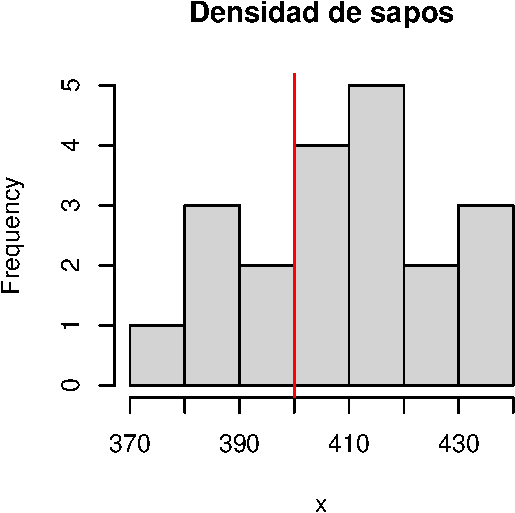
\includegraphics{Pruebas-hipotesis_files/figure-beamer/unnamed-chunk-1-1.pdf}
\#\#\# Ejemplo

Visualmente, pareciera que la media reportada en literatura, es menor
que la econtrada. Necesitamos, sin embargo, ver si esta apreciación
visual es estadísticamente válida, por lo que trataremos de rechazar la
siguiente hipótesis estadística nula:

\$H\_0 = \$ La densidad de renacuajos promedio estimada en campo es
igual a la reportada en la literatura
\end{frame}

\begin{frame}{Ejemplo}
\protect\hypertarget{ejemplo-5}{}
Alternativas:

\begin{itemize}
\item
  Calcular intervalos de confianza al 95\%
\item
  Ver si valor reportado está dentro del intervalo
\end{itemize}
\end{frame}

\begin{frame}[fragile]{Ejemplo}
\protect\hypertarget{ejemplo-6}{}
Haciendo los cálculos en R

\begin{Shaded}
\begin{Highlighting}[]
\NormalTok{media }\OtherTok{\textless{}{-}} \FunctionTok{mean}\NormalTok{(x)}
\NormalTok{desv }\OtherTok{\textless{}{-}} \FunctionTok{sd}\NormalTok{(x)}
\NormalTok{n }\OtherTok{\textless{}{-}} \FunctionTok{length}\NormalTok{(x)}
\end{Highlighting}
\end{Shaded}

Intervalos:

\begin{Shaded}
\begin{Highlighting}[]
\NormalTok{media }\SpecialCharTok{+} \FloatTok{1.96} \SpecialCharTok{*}\NormalTok{ desv }\SpecialCharTok{/} \FunctionTok{sqrt}\NormalTok{(n)}
\end{Highlighting}
\end{Shaded}

\begin{verbatim}
## [1] 416.0556
\end{verbatim}

\begin{Shaded}
\begin{Highlighting}[]
\NormalTok{media }\SpecialCharTok{{-}} \FloatTok{1.96} \SpecialCharTok{*}\NormalTok{ desv }\SpecialCharTok{/} \FunctionTok{sqrt}\NormalTok{(n)}
\end{Highlighting}
\end{Shaded}

\begin{verbatim}
## [1] 399.8444
\end{verbatim}
\end{frame}

\begin{frame}{Ejemplo}
\protect\hypertarget{ejemplo-7}{}
Podemos ver que la media reportada está dentro del intervalo

\[IC_{95} = \{399.8, 416.1\}\]

Por lo tato, la probabilidad de que la media reportada sea igual a la
media encontrada es

\(P > 0.05\)

Con lo cual aceptamos \(H_0\)
\end{frame}

\end{document}
